\documentclass[11pt]{article}
\usepackage[margin=1in]{geometry}
\usepackage[T1]{fontenc}
\usepackage{lmodern,amsmath,amssymb,amsthm,mathtools,booktabs,longtable,array,graphicx}
\usepackage[dvipsnames]{xcolor}
\usepackage[colorlinks=true,linkcolor=MidnightBlue,urlcolor=MidnightBlue,citecolor=MidnightBlue]{hyperref}
\usepackage{microtype,fancyhdr}
\graphicspath{{figures/}{astra_fresh_p1_20261023/figures/}}
\pagestyle{fancy}\fancyhf{}\fancyhead[L]{ASTRA FRESH \quad P1 \quad Private research}
\fancyhead[R]{23 October 2026}\fancyfoot[C]{\thepage}
\setlength{\headheight}{14pt}
\newtheorem{theorem}{Theorem}[section]
\newtheorem{lemma}[theorem]{Lemma}
\newtheorem{corollary}[theorem]{Corollary}
\newtheorem{proposition}[theorem]{Proposition}
\theoremstyle{remark}\newtheorem{remark}[theorem]{Remark}
\newcommand{\R}{\mathbb R}
\newcommand{\one}{\mathbf 1}
\newcommand{\op}{\mathrm{op}}
\newcommand{\F}{\mathrm F}
\newcommand{\SG}{\mathcal S_G}
\newcommand{\M}{\mathcal M}
\newcommand{\Pp}{\mathsf P}
\newcommand{\diag}{\operatorname{diag}}
\newcommand{\tr}{\operatorname{tr}}
\newcommand{\range}{\operatorname{range}}
\newcommand{\norm}[1]{\left\lVert #1\right\rVert}
\newcommand{\ip}[2]{\left\langle #1,#2\right\rangle}
\title{Green diagonals and local cycle probes\\for stable sparse matrix recovery}
\author{Astra P1 --- foundational mathematics\\ASTRA-FRESH-20261023, Prompt 1.1}
\date{23 October 2026 \quad Version 1.0 \quad Private, disclosure not cleared}
\begin{document}
\maketitle
\begin{abstract}
We derive an exact representation of the normal operator for regular-simplex probing of a known sparse symmetric matrix. The representation separates two stability questions. Frobenius stability is controlled by the smallest eigenvalue of a grounded graph Laplacian, whereas operator-norm stability is equivalent, up to constants depending only on the fixed probe count, to bounded diagonal entries of its inverse. We prove explicit lattice dimension thresholds and construct full cubic supports recoverable from three row-normalized matrix actions with a dimension-independent operator error bound, even though their Frobenius inverse constants grow as the square root of dimension. A change of probe direction at one vertex, together with three local cycle functionals, removes a genuine global ambiguity. The full-support decoder requires one grounded-Laplacian solve. The mathematical statements below are proved in this note; the only non-elementary existence input is a checked random-lift eigenvalue theorem. Floating-point diagnostics, originality, and technological advantage are separate claims. Priority is UNKNOWN; independent proof review and practical advantage are not established.
\end{abstract}

\section{Contract, scope, and provenance}

Let $G=(V,E)$ be a known finite simple graph, with $|V|=n$ and $|E|=m$. Define
\[
\SG=\{H\in\R^{n\times n}: H^T=H,\ H_{ij}=0\text{ for }i\ne j,\ ij\notin E\}.
\]
Every diagonal entry and every permitted edge entry is arbitrary and unknown. In particular, we assume neither positivity nor a bound on the entries or the norm of $H$. A fixed probe matrix $X\in\R^{n\times q}$ is chosen using the graph, with the \emph{whole-row} normalization
\[
\norm{X_{i,:}}_2\leq 1\qquad(i\in V).
\]
The data are $Y=HX+E_0$, where $E_0$ is arbitrary and $\norm{E_0}_{\F}\leq\varepsilon$. The target is an absolute guarantee
\[
\norm{\widehat H-H}_{\op}\leq C\varepsilon
\]
with $C$ independent of $n$. The number $q$ counts matrix--vector actions, not individual scalar observations. Exact real arithmetic and exact support are part of the theorem's contract. Finite-precision stability is an additional question.

The primary corpus was read beginning with \texttt{00\_START\_HERE.txt} at revision
\begin{center}\small\texttt{e606bfc587c76bdcae8b8fa3ec33e721efa2fbac}.\end{center}
The repository's \texttt{AGENTS.md} was also read. The scientific material selected from the archive was the cycle-11 Pro2 proof's matrix-action contract, especially the distinction between a Frobenius sufficient bound and an operator-norm target \cite{corpus}. That historical Pro2 label does not identify the fresh programme's physical-invention branch. No result from a current sibling branch is assumed. This note does not settle the archive's general treewidth-two, degree-four, four-query problem.

\paragraph{What is proved here.}
The strongest scoped result is an exact Green-diagonal characterization for a particular family of probes, followed by a complete three-query construction on an infinite family of full cubic supports. The construction is not a universal method for arbitrary sparse matrices. The underlying inverse-problem viewpoint and graph-coloring recovery are established subjects; no claim of first use of those ideas is made.

\section{The simplex normal operator}

Fix $q\geq1$. Suppose $\Delta(G)\leq q$ and there is a coloring
$c:V\to\{0,\ldots,q\}$ that is injective on every closed neighborhood $N[i]$.
Let $v_0,\ldots,v_q\in\R^q$ be a unit regular simplex:
\[
\ip{v_a}{v_b}=\begin{cases}1&a=b,\\-1/q&a\ne b,\end{cases}
\qquad \sum_{a=0}^qv_a=0.
\]
Set $X_{i,:}=v_{c(i)}^T$. Each row has norm exactly one. Write $A$ for adjacency,
$D=\diag(d_i)$ for degree, and $L=D-A$ for the graph Laplacian. Introduce
\begin{equation}\label{eq:B}
B=2qI-D-A=L+2\diag(q-d_i).
\end{equation}
Use the Frobenius inner product on $\SG$; its orthonormal coordinates are $H_{ii}$ and $\sqrt2H_{ij}$ for $ij\in E$. Define $S:\SG\to\R^n$ by $S(H)=H\one$.

\begin{theorem}[Exact normal operator and spectrum]\label{thm:normal}
For $\M(H)=HX$,
\begin{align}
\norm{HX}_{\F}^2&=\frac{q+1}{q}\norm H_{\F}^2-\frac1q\norm{H\one}_2^2,\label{eq:energy}\\
N:=\M^*\M&=\frac{q+1}{q}I_{\SG}-\frac1q S^*S.\label{eq:normal}
\end{align}
The spectrum of $N$, with multiplicity, consists of
\[
\frac{\lambda_1(B)}{2q},\ldots,\frac{\lambda_n(B)}{2q},
\qquad \frac{q+1}{q}\quad\text{repeated }m\text{ times}.
\]
The measurement is injective if and only if every connected component has a vertex of degree less than $q$. In this case
\begin{equation}\label{eq:inverse}
N^{-1}=\frac q{q+1}\bigl(I_{\SG}+2S^*B^{-1}S\bigr).
\end{equation}
\end{theorem}

\begin{proof}
For each row $i$, the nonzero coordinates of $H_{i,:}$ multiply distinct simplex vertices. Their Gram matrix is $(q+1)I/q-\one\one^T/q$. Summing the resulting row energies gives \eqref{eq:energy}; polarization gives \eqref{eq:normal}.
The adjoint $S^*$ satisfies
\[
(S^*a)_{ii}=a_i,\qquad(S^*a)_{ij}=(a_i+a_j)/2\quad(ij\in E).
\]
Consequently
\begin{equation}\label{eq:SS}
SS^*=I+(D+A)/2=(q+1)I-B/2.
\end{equation}
Since the diagonal coordinates make $S$ surjective, $S^*S$ has these $n$ nonzero eigenvalues and $m$ zero eigenvalues. This proves the spectral statement. Moreover,
\begin{equation}\label{eq:Benergy}
a^TBa=\sum_{ij\in E}(a_i-a_j)^2+2\sum_i(q-d_i)a_i^2.
\end{equation}
It vanishes precisely for vectors constant on each component and zero on components with a degree defect. Thus $B$ is positive definite exactly under the stated condition. On a $q$-regular component the nonzero matrix $I+A$ is in $\ker\M$, since each closed neighborhood contains the whole simplex. Finally substitute \eqref{eq:SS} into the product of \eqref{eq:normal} and the proposed inverse; the coefficients of $S^*(\cdot)S$ cancel.
\end{proof}

\paragraph{A concrete decoder.}
Let $\Pp_G$ be Frobenius-orthogonal projection onto $\SG$; it symmetrizes and deletes unsupported entries. For arbitrary $Y$, compute
\begin{equation}\label{eq:decoder}
Z=\M^*Y=\Pp_G(YX^T),\qquad Ba=Z\one,\qquad
\mathcal D_G(Y)=\frac q{q+1}(Z+2S^*a).
\end{equation}
This is canonical least squares. It uses one $n$-dimensional positive-definite solve, plus supported matrix operations. No unknown entry of $H$ is supplied to the decoder. Sparse factorization fill and iterative-solver precision are not bounded by this identity alone.

\section{The norm that carries the difficulty}

Assume $B>0$, set $\mathcal G=B^{-1}$, and let $g=\max_i\mathcal G_{ii}$. Define
\[
\kappa_{\op}=\sup_{0\ne H\in\SG}\frac{\norm H_{\op}}{\norm{HX}_{\F}},\qquad
\kappa_{\F}=\sup_{0\ne H\in\SG}\frac{\norm H_{\F}}{\norm{HX}_{\F}}.
\]

\begin{theorem}[Green-diagonal criterion]\label{thm:green}
For $\norm u_2=1$, put $K_u=\Pp_G(uu^T)$ and $b(u)=S K_u$. Then
\begin{equation}\label{eq:variational}
\kappa_{\op}^2=\frac q{q+1}\sup_{\norm u_2=1}
\left(\norm{K_u}_{\F}^2+2b(u)^T\mathcal G b(u)\right).
\end{equation}
In particular,
\begin{equation}\label{eq:kappa-bounds}
\frac q{q+1}(1+2g)\ \leq\ \kappa_{\op}^2\ \leq\
\frac q{q+1}\bigl(1+2(q+1)^2g\bigr).
\end{equation}
For fixed $q$, a family of these designs is uniformly operator stable if and only if its maximum Green diagonal is uniformly bounded. In contrast,
\begin{equation}\label{eq:kappaF}
\kappa_{\F}=\sqrt{\frac{2q}{\lambda_{\min}(B)}}.
\end{equation}
The decoder \eqref{eq:decoder} has worst-case noise amplification exactly $\kappa_{\op}$ in the operator target norm. No decoder exact on all noiseless data for this fixed $X$ has a smaller uniform absolute amplification constant.
\end{theorem}

\begin{proof}
For symmetric $H$, $\norm H_{\op}=\sup_{\norm u_2=1}|u^THu|$ and
$u^THu=\ip{K_u}{H}$. In a positive-definite quadratic norm $\ip H{NH}$, the squared dual norm of $K_u$ is $\ip{K_u}{N^{-1}K_u}$. Interchanging the two suprema and using \eqref{eq:inverse} proves \eqref{eq:variational}.

We have $\norm{K_u}_{\F}\leq\norm{uu^T}_{\F}=1$. Entrywise,
\[
b_i(u)=u_i\left(u_i+\sum_{j\sim i}u_j\right),\qquad
\norm{b(u)}_1\leq1+2\sum_{ij\in E}|u_iu_j|\leq q+1.
\]
Positive semidefiniteness of $\mathcal G$ implies
$|\mathcal G_{ij}|\leq\sqrt{\mathcal G_{ii}\mathcal G_{jj}}\leq g$. Thus
$b^T\mathcal G b\leq g\norm b_1^2$, proving the upper bound. For the lower bound use $u=e_i$ at a largest diagonal: then $K_u=e_ie_i^T$ and $b=e_i$. The spectral statement in Theorem~\ref{thm:normal} gives \eqref{eq:kappaF}; indeed $B\preceq2qI$ because $D+A$ is positive semidefinite.

For arbitrary noise, $\M\mathcal D_G(E_0)$ is its orthogonal projection onto $\range\M$. Hence
$\norm{\mathcal D_G(E_0)}_{\op}\leq\kappa_{\op}\norm{E_0}_{\F}$.
Conversely take true matrix zero and noise $E_0=\M(H)$. Every noiseless-exact decoder must output $H$ on these data. Taking the supremum proves optimality, without assuming the competing decoder is linear.
\end{proof}

\paragraph{Capacity interpretation, without an imported theorem.}
For each vertex,
\begin{equation}\label{eq:capacity}
\frac1{\mathcal G_{ii}}=\min_{a_i=1}a^TBa.
\end{equation}
To prove it, use Cauchy--Schwarz in the $B$ inner product:
$1=\ip{a}{B^{-1}e_i}_B^2\leq(a^TBa)\mathcal G_{ii}$; equality is attained at
$a=B^{-1}e_i/\mathcal G_{ii}$. Equation~\eqref{eq:Benergy} is the energy of unit-conductance graph edges and ground conductance $2(q-d_i)$ at each vertex. Thus the relevant invariant is a local grounded resistance, or equivalently a local capacity. A small global eigenvalue alone cannot decide the operator-norm question.

\section{One deleted edge and an effective-resistance formula}

Let $F$ be a connected $q$-regular graph with the same local coloring, and delete an edge $ab$ to obtain $G$. Write $L_0=qI-A_F$, $s=e_a+e_b$, and $L_0^+$ for the Moore--Penrose inverse. The deleted edge is a known zero only in this section; Section~\ref{sec:full} removes that restriction.

\begin{theorem}[Rank-one grounding]\label{thm:rank-one}
\begin{align}
B_G&=L_0+ss^T,\label{eq:rankone}\\
B_G^{-1}&=(I-\one s^T/2)L_0^+(I-s\one^T/2)+\one\one^T/4.\label{eq:green-rankone}
\end{align}
If $R_{ij}=(e_i-e_j)^TL_0^+(e_i-e_j)$, then
\begin{equation}\label{eq:resistance}
(B_G^{-1})_{ii}=\frac14+\frac{R_{ia}+R_{ib}}2-\frac{R_{ab}}4.
\end{equation}
If $\lambda_2(L_0)\geq\gamma>0$, then
\begin{equation}\label{eq:expander-g}
g\leq\frac14+\frac3{2\gamma},\qquad
\kappa_{\F}\geq\sqrt{qn/2}.
\end{equation}
For a fixed positive gap, $\kappa_{\op}=O_q(1)$ and $\kappa_{\F}=\Theta_q(\sqrt n)$, with constants also depending on the gap.
\end{theorem}

\begin{proof}
Deleting $ab$ decreases both endpoint degrees by one and removes both adjacency entries, giving \eqref{eq:rankone}. To solve $(L_0+ss^T)a=f$, multiplication by $\one^T$ gives $s^Ta=\one^Tf/2$. Therefore
$L_0a=(I-s\one^T/2)f$. Its mean-zero solution, plus the unique constant satisfying the previous constraint, is \eqref{eq:green-rankone}.
The diagonal is $1/4+(e_i-s/2)^TL_0^+(e_i-s/2)$; expanding gives \eqref{eq:resistance}. The vector in this quadratic form is mean zero and has squared norm at most $3/2$, proving the first bound in \eqref{eq:expander-g}. The Rayleigh quotient of $B_G$ at $\one$ is $4/n$, proving the second. Finally $\lambda_{\max}(B_G^{-1})\leq\tr(B_G^{-1})\leq ng$ supplies the matching Frobenius upper order.
\end{proof}

\paragraph{Several deleted edges.}
If a nonempty set $T$ of edges is deleted from $F$, then
\begin{equation}\label{eq:multiground}
B_{F\setminus T}=L_0+\sum_{ab\in T}(e_a+e_b)(e_a+e_b)^T.
\end{equation}
It is positive definite and dominates the matrix for any single edge in $T$. Inversion reverses positive-definite order, so the same upper bound on $g$ holds. No connectivity assumption on $F\setminus T$ is needed.

\section{A lattice threshold, including the logarithmic case}

Let $F=(\mathbb Z/\ell\mathbb Z)^d$ with nearest-neighbor edges, $q=2d$, and
$\ell\geq3$ divisible by $2d+1$. The coloring
\[
c(x)=\sum_{j=1}^d jx_j\pmod{2d+1}
\]
is locally injective: the closed-neighborhood increments are $0,\pm1,\ldots,\pm d$. Delete one nearest-neighbor edge and use the simplex design.

\begin{theorem}[Dimension threshold]\label{thm:torus}
As $\ell\to\infty$ through the stated multiples, with $d$ fixed,
\begin{center}
\begin{tabular}{ccc}\toprule
Dimension & $\kappa_{\op}$ & $\kappa_{\F}$\\\midrule
$d=1$ & $\Theta(\sqrt\ell)$ & $\Theta(\ell)$\\
$d=2$ & $\Theta(\sqrt{\log\ell})$ & $\Theta(\ell\sqrt{\log\ell})$\\
$d\geq3$ & $\Theta(1)$ & $\Theta(\ell^{d/2})$\\\bottomrule
\end{tabular}
\end{center}
These are laws for these specified probes, not lower bounds against all other probe designs on the same support.
\end{theorem}

\begin{proof}
Fourier characters diagonalize $L_0$, with eigenvalues
\[
\lambda(k)=4\sum_{j=1}^d\sin^2(\pi k_j/\ell).
\]
Its pseudoinverse has constant diagonal
\[
S_\ell=\ell^{-d}\sum_{k\ne0}\frac1{\lambda(k)}.
\]
For representatives $|k_j|\leq\ell/2$, the inequalities
$2|k_j|/\ell\leq|\sin(\pi k_j/\ell)|\leq\pi|k_j|/\ell$ show that
$S_\ell$ is comparable, with dimension-dependent constants, to
$\ell^{2-d}\sum_{0<\norm k_\infty\leq\ell/2}\norm k_2^{-2}$.
There are $\Theta_d(r^{d-1})$ integer points in the sup-norm shell $r$ and their squared Euclidean norms lie between $r^2$ and $dr^2$. Summing $r^{d-3}$ gives
\[
S_\ell=\begin{cases}\Theta(\ell)&d=1,\\\Theta(\log\ell)&d=2,\\\Theta(1)&d\geq3.\end{cases}
\]
For adjacent $a,b$, translation and coordinate symmetries make $R_{ab}$ the same on all edges. Since
$\sum_{ab\in E(F)}R_{ab}=\tr(L_0^+L_0)=n-1$, it equals $(n-1)/(dn)\leq1$.
Average \eqref{eq:resistance} over $i$, using $L_0^+\one=0$ and constant diagonal, to obtain
\[
\frac1n\tr(B_G^{-1})=\frac14+2S_\ell-R_{ab}/4.
\]
The diagonal formula and $|(L_0^+)_{ij}|\leq S_\ell$ give
\begin{equation}\label{eq:torusg}
2S_\ell\leq g\leq\frac14+4S_\ell.
\end{equation}
Moreover the Rayleigh quotient of $B_G^{-1}$ at $\one$ is
$n(1/4+S_\ell-R_{ab}/4)$, between one half of its trace and its trace. Hence
$\lambda_{\max}(B_G^{-1})=\Theta(n(1+S_\ell))$.
Apply Theorem~\ref{thm:green} to obtain every entry of the table.
\end{proof}

\section{Local cycle measurements and full support}\label{sec:full}

For a connected regular cover $F$, the unmodified probe has the exact ambiguity
\[
H_0=I+A_F,\qquad H_0X_0=0,\qquad\norm{H_0}_{\op}=q+1,
\quad\norm{H_0}_{\F}=\sqrt{(q+1)n}.
\]
Changing only the \emph{magnitude} of a probe row cannot remove it. If $X=DX_0$ for invertible diagonal $D$, then $D^{-1}H_0D^{-1}$ is a nonzero supported symmetric null matrix. A change of projective direction is essential.

\begin{lemma}[Cycle witness]\label{lem:cycle}
Give a simple cycle $C$ of length $r$ an orientation, and put
\[
Z_i=\frac{v_{c(i_+)}-v_{c(i_-)}}{\sqrt{2r(q+1)/q}}\quad(i\in C),\qquad Z_i=0\quad(i\notin C),
\]
where $i_+$ and $i_-$ are the next and previous cycle vertices. Then $\norm Z_{\F}=1$ and $\M_0^*Z=0$ on the full supported symmetric space. Suppose $C\cap N[v]=\{u\}$ and put
\[
h=\frac{v_{c(u_+)}-v_{c(u_-)}}{\sqrt{2(q+1)/q}},\quad
X_t=X_0+t e_vh^T.
\]
Then $h\perp X_{0,v,:}$ and, for every supported symmetric $H$,
\begin{equation}\label{eq:anchor}
\ip Z{HX_t}=\frac{t}{\sqrt r}H_{uv}.
\end{equation}
\end{lemma}

\begin{proof}
Let $f_{ij}=1$ on forward cycle edges, $-1$ on backward edges, and zero elsewhere. It is antisymmetric and has zero divergence. Before normalization, $Z_i=\sum_jf_{ij}v_{c(j)}$. Thus $\ip{v_{c(i)}}{Z_i}=0$ and, on every graph edge,
$\ip{v_{c(j)}}{Z_i}=(q+1)f_{ij}/q$. The two endpoint terms cancel in the symmetric measurement adjoint. Each nonzero row has squared norm $2(q+1)/q$, proving the normalization. Local injectivity and the separation of the cycle from $v$ make its two neighbor colors distinct from $c(v)$, so $h\perp X_{0,v,:}$. Finally the perturbation contributes $t\sum_iH_{iv}\ip{Z_i}{h}$; only $i=u$ survives, with pairing $1/\sqrt r$.
\end{proof}

\begin{proposition}[One-cycle extension with a small perturbation]\label{prop:onecycle}
Under Lemma~\ref{lem:cycle}, let $\mathcal D$ be the simplex least-squares decoder for $G=F-uv$, and let $K$ bound its Frobenius-to-operator norm. If $0<t<1/K$, then $X=X_t/\rho$, $\rho=\sqrt{1+t^2}$, admits a linear exact decoder with noise bound
\begin{equation}\label{eq:small-bound}
C\leq\frac{\rho}{1-tK}\left(K+\frac{(q+1)\sqrt r}{t}\right).
\end{equation}
It can be implemented with grounded solves and a $(q+1)$-dimensional correction system. The sufficient condition is on $K$, not on the smallest nonzero Frobenius singular value of the regular measurement.
\end{proposition}

\begin{proof}
Let $T(H)=He_vh^T$. For all full-support $H$,
\[
\mathcal D(HX_0)=H-H_{uv}H_0.
\]
Indeed $H-H_{uv}H_0$ has zero $uv$ entry and the same unmodified data. For unscaled data $Y_t=HX_t$ set
$\beta=\sqrt r\ip Z{Y_t}/t$ and $w=\mathcal D(Y_t)+\beta H_0$. Then
$w=(I+t\mathcal DT)H$. Since $\norm{T(H)}_{\F}=\norm{He_v}_2\leq\norm H_{\op}$, the Neumann bound gives invertibility and \eqref{eq:small-bound}. The formula defines a bounded linear left inverse on arbitrary noisy data as well. The range of $T$ has dimension at most $q+1$; Woodbury reduction gives the stated implementation.
\end{proof}

This proposition already covers full three-dimensional tori using a square beyond a neighbor of the changed vertex, since their $L_0^+$ diagonals are bounded. A stronger, nonperturbative construction is available for the cubic family below.

\subsection{Triangle expansion of a bipartite cubic graph}

Start with a connected simple cubic bipartite graph $J=(L,R,E_J)$ and a proper edge coloring by $1,2,3$. Replace each right vertex $r$ by a triangle with port colors $1,2,3$. Keep the left vertices and give them color zero. Replace a base edge of color $c$ by an edge from its left endpoint to port $c$ in the corresponding triangle. The resulting graph $F$ is cubic, and every closed neighborhood has all four colors. Each left vertex has neighbors in three distinct, disjoint triangles.

\begin{lemma}[Gap transfer]\label{lem:gap}
If the unnormalized Laplacian gap of $J$ is at least $\gamma_J>0$, then the gap of $F$ is at least
\begin{equation}\label{eq:gaptransfer}
\gamma_F\geq\frac1{6/\gamma_J+1/3}.
\end{equation}
\end{lemma}

\begin{proof}
For a function on $F$, write $x_l$ for left values and $y_{r,c}$ for port values; put $m_r=\frac13\sum_cy_{r,c}$. Let $E_\times$ and $E_\triangle$ be its cross-edge and triangle energies. Then
$E_\triangle=3\sum_{r,c}(y_{r,c}-m_r)^2$. The function $g=(x_l,m_r)$ on $J$ has energy
$E_J(g)\leq2E_\times+(2/3)E_\triangle\leq2(E_\times+E_\triangle)$.
Choose $a$ to be the mean of $g$ on $J$. Its squared deviation on $F$ is at most
$3\sum_{J}(g-a)^2+E_\triangle/3$, hence at most
$(6/\gamma_J+1/3)(E_\times+E_\triangle)$. Minimizing over constants on $F$ proves the Poincare inequality and the gap claim.
\end{proof}

\subsection{Three cycle functionals recover the whole changed column}

Choose a left vertex $v$ and call its port neighbors $u_1,u_2,u_3$ in color order. Let $C_j$ be the triangle of $u_j$. Orient each with $u_j$ first and use the unit cycle witnesses $Z_j$ of Lemma~\ref{lem:cycle}. Their supports are disjoint, so the three witnesses are orthonormal in the data Frobenius inner product. Choose
\[
h=(v_2-v_3)/\sqrt{8/3},\qquad X_t=X_0+t e_vh^T,\qquad X=X_t/\rho.
\]
Let $c_j=\ip{Z_{j,u_j,:}}h$. The absolute values are
\begin{equation}\label{eq:pairings}
|c_1|=1/\sqrt3,\qquad |c_2|=|c_3|=1/(2\sqrt3).
\end{equation}
The orientation determines the signs, which are known. For $Y_t=\rho Y$, define
\begin{equation}\label{eq:beta}
\widehat\beta_j=\frac{\ip{Z_j}{Y_t}}{tc_j}.
\end{equation}
In noiseless data these are precisely the three unknown entries $H_{vu_j}$.

Let $F_\beta$ be the symmetric star matrix with those three entries and zero elsewhere. Let $G_*$ be $F$ with all three edges at $v$ deleted, retaining every vertex and all diagonal entries. Define a data-row map $Q$ by leaving every row except $v$ unchanged and replacing row $v$ with
\begin{equation}\label{eq:rowmap}
(QW)_{v,:}=\frac{\ip{W_{v,:}}{(X_t)_{v,:}}}{\rho^2}X_{0,v,:}.
\end{equation}
This is a contraction in Frobenius norm. The complete decoder is
\begin{equation}\label{eq:star-decoder}
\widehat H=\mathcal D_{G_*}\bigl(Q(Y_t-F_{\widehat\beta}X_t)\bigr)+F_{\widehat\beta}.
\end{equation}

\begin{theorem}[Full cubic recovery, without a small-perturbation condition]\label{thm:full}
For every $t>0$, \eqref{eq:star-decoder} is exact on all noiseless matrices supported on the full graph $F$. It uses three actions satisfying the whole-row budget. If $K$ bounds the Frobenius-to-operator norm of $\mathcal D_{G_*}$, then for arbitrary noise
\begin{equation}\label{eq:star-bound}
\norm{\widehat H-H}_{\op}\leq
\rho\left[K+\left(1+K\sqrt{\rho^2+4/3}\right)\frac{2\sqrt3}{t}\right]\norm{E_0}_{\F}.
\end{equation}
At $t=1$, the displayed constant is
\begin{equation}\label{eq:t1bound}
(\sqrt2+4\sqrt5)K+2\sqrt6.
\end{equation}
Each decoder call uses three cycle inner products, local star operations, and one grounded-Laplacian solve.
\end{theorem}

\begin{proof}
The cycle calculation gives \eqref{eq:beta}. Set $H'=H-F_\beta$. Its only possibly nonzero entry in column $v$ is its diagonal. Thus
$Q(H'X_t)=H'X_0$, giving exactness of \eqref{eq:star-decoder}.

For noise write $E_t=\rho E_0$ and $\delta\beta=\widehat\beta-\beta$. Orthonormality of the three cycle witnesses and \eqref{eq:pairings} imply
\[
\norm{\delta\beta}_2\leq\frac{2\sqrt3}{t}\norm{E_t}_{\F}.
\]
The star matrix has operator norm $\norm{F_{\delta\beta}}_{\op}=\norm{\delta\beta}_2$. Its data satisfy
\[
\norm{F_{\delta\beta}X_t}_{\F}^2
=\norm{\textstyle\sum_j\delta\beta_j v_j}_2^2+\rho^2\norm{\delta\beta}_2^2
\leq(4/3+\rho^2)\norm{\delta\beta}_2^2,
\]
since the three-neighbor simplex Gram matrix is $4I/3-\one\one^T/3$.
Subtract the noiseless reconstruction from \eqref{eq:star-decoder}, use $\norm Q\leq1$, and apply the internal decoder bound. This gives \eqref{eq:star-bound}. Every step is linear in the measured data.
\end{proof}

\subsection{An infinite family with a fixed constant}

\begin{corollary}[Three actions are optimal on a full-support family]\label{cor:family}
For every sufficiently large integer $s$, there exists a simple cubic support graph on $n=12s$ vertices and an explicit probe/decoder construction as above such that
\[
\norm{\widehat H-H}_{\op}\leq550\norm{E_0}_{\F}
\]
for every supported symmetric $H$ and every noise matrix. Two actions cannot exactly recover every member, even with deterministic adaptive queries. For the three-query design at $t=1$,
\[
\kappa_{\F}\geq\sqrt{2n},\qquad\kappa_{\F}=\Theta(\sqrt n),
\]
whereas its operator inverse constant is bounded independently of $n$.
\end{corollary}

\begin{proof}
Use a random $s$-lift of $K_{3,3}$ as $J$. It is simple, bipartite, and cubic. The edge coloring $c(i,j)=j-i\pmod3$ (shifted to $1,2,3$) on $K_{3,3}$ lifts to a proper coloring. Bordenave's Corollary 24 states that the largest absolute new adjacency eigenvalue of a random lift of a fixed $d$-regular graph is at most $2\sqrt{d-1}+\eta$ with probability tending to one, for every fixed $\eta>0$ \cite{bordenave}. The old spectrum of $K_{3,3}$ is $3,-3,0,0,0,0$. Choose $\eta=3-2\sqrt2-0.08>0$. Then, for all sufficiently large $s$, a lift with Laplacian gap at least $0.08$ exists. Such a lift is connected; the retained eigenvalue $-3$ from bipartiteness does not reduce the positive Laplacian gap.

Triangle expansion yields $n=12s$ and $\gamma_F\geq3/226$ by Lemma~\ref{lem:gap}. By \eqref{eq:multiground}, the star-deletion decoder has
\[
g\leq\frac14+\frac3{2\gamma_F}\leq113.25,\qquad
K^2\leq\tfrac34(1+32g)\leq2718.75.
\]
Equation~\eqref{eq:t1bound} is therefore at most $545.008<550$.
The generator is explicit given a base graph; the cited theorem supplies the existence of suitable bases, not a deterministic gap certificate for every random sample.

For the lower bound use $H_0=I+A_F$. Only the changed row of the probe breaks its ambiguity, so
\[
\norm{H_0X}_{\F}=\frac t\rho\norm{H_0e_v}_2
=\frac{2t}{\rho},\qquad
\frac{\norm{H_0}_{\F}}{\norm{H_0X}_{\F}}=\frac{\rho\sqrt n}{t}.
\]
At $t=1$ this is $\sqrt{2n}$. Conversely $\norm H_{\F}\leq\sqrt n\norm H_{\op}$ and the operator guarantee give the matching upper order for the inverse constant.

The full supported space has dimension $n+3n/2=5n/2>2n$. Along the zero-data transcript, two deterministic adaptive actions impose at most $2n$ homogeneous linear constraints on this space. A nonzero matrix satisfies both and is indistinguishable from zero. Thus two queries cannot give exact recovery for all inputs. This argument does not assert a probabilistic lower bound for a different randomized approximate-recovery contract.
\end{proof}

\paragraph{Baseline and significance.}
Four one-hot color probes on the same locally colored graph satisfy
$\norm{HX}_{\F}=\norm H_{\F}$ and have a Frobenius-contractive least-squares decoder. The present result saves one action while accepting larger constants. No speedup, lower end-to-end cost, or superiority to all other three-query designs has been established. The mathematically substantive separation is that a diverging Frobenius inverse constant is compatible with uniform operator stability, even at the minimum exact query count on these full supports.

\section{An inexact-solve certificate}

The next implementation issue can be resolved at the level of a posteriori residuals without changing the measurement theorem. In \eqref{eq:decoder}, let $\widetilde a$ be an approximate solve and define its true residual $r=Z\one-B\widetilde a$. The difference between the approximate and exact decoded matrices is
\[
\Delta H=-\frac{2q}{q+1}S^*B^{-1}r.
\]
Because $\norm{S^*a}_{\op}\leq(q+1)\norm a_\infty$, positive semidefiniteness of $B^{-1}$ gives the computable sufficient bound
\begin{equation}\label{eq:residual-l1}
\norm{\Delta H}_{\op}\leq2qg\norm r_1.
\end{equation}
An energy alternative is $2q\sqrt g\sqrt{r^TB^{-1}r}$, though evaluating or certifying the latter requires additional solver information. Thus, with a certified upper bound on $g$, an absolute $\ell_1$ residual tolerance gives a dimension-independent operator error certificate. This is a conditional numerical certificate: the residual itself must be evaluated with controlled roundoff.

For the regular-parent constructions there is also a useful balanced $\ell_2$ certificate. Suppose $B=L_0+\sum_{e\in T}s_es_e^T$, $s_e=e_a+e_b$, $k=|T|\geq1$, $b=\sum_{e\in T}s_e$, and $\lambda_2(L_0)\geq\gamma$. If $\one^Tr=0$, write $a=B^{-1}r=w+c\one$ with $w\perp\one$. Multiplying the equation by $\one^T$ gives $b^Ta=0$, whence $c=-b^Tw/(2k)$. The energy inequality yields
\[
\gamma\norm w_2^2\leq a^TBa=a^Tr=w^Tr\leq\norm w_2\norm r_2.
\]
Consequently
\begin{equation}\label{eq:balanced}
\norm{\Delta H}_{\op}\leq\frac{2q}{\gamma}
\left(1+\frac{\norm b_2}{2k}\right)\norm r_2.
\end{equation}
Any candidate solve can be balanced by the scalar correction
\[
\widetilde a\longleftarrow\widetilde a+\frac{\one^Tr}{4k}\one,
\qquad r\longleftarrow r-\frac{\one^Tr}{2k}b.
\]
The corrected residual has zero sum in exact arithmetic, and its actual norm is used in \eqref{eq:balanced}.

The balance condition matters. In the one-edge case, a unit-$\ell_2$ residual $r=\one/\sqrt n$ has
\[
\frac1n\one^TB^{-1}r=\frac{\sqrt n}{4}(1+s^TL_0^+s)\geq\frac{\sqrt n}{4}.
\]
Some diagonal of $S^*B^{-1}r$ therefore has magnitude at least $\sqrt n/4$, so the corresponding decoded error is at least $q\sqrt n/[2(q+1)]$. A uniform bound based solely on an unbalanced $\ell_2$ residual is false even when $g$ is bounded. Equations~\eqref{eq:residual-l1} and \eqref{eq:balanced} retain exactly the missing information. They do not yet prove an end-to-end floating-point complexity bound.

\section{Implementation, attempted falsification, and numerical evidence}

The archive contains \texttt{recovery.py}, \texttt{anchored.py}, four verification scripts, exact graph edge/color records, and JSON results. The seeds are recorded in those results. The diagnostics use Python 3.12.14, NumPy 2.3.5, and SciPy 1.17.0 with one BLAS/OpenMP thread. They are producer-run floating-point checks, not independent, formal, or interval-certified proofs.

\begin{center}\small
\begin{tabular}{p{0.32\textwidth}p{0.30\textwidth}p{0.28\textwidth}}\toprule
Check & Scope & Result\\\midrule
Normal matrix, spectrum, inverse & Seven small graphs, including disconnected support & All stated tolerances passed\\
One-edge grounding formula & $K_4$ lifts through $n=1024$ & Largest-instance max error $4.1\cdot10^{-14}$\\
One-cycle full-support decoder & Triangle covers through $n=768$ & Largest relative recovery error $4.0\cdot10^{-14}$\\
Nonperturbative full-support decoder & Eight sizes through $n=1536$ & Largest-instance relative error $5.8\cdot10^{-15}$\\
Cycle-noise adversary & Full support, $n=1536$, unit data noise & Operator error $14.74$\\
Old-kernel adversary & Same instance & Frobenius gain $55.4256=\sqrt{2n}$\\
Torus Fourier formulas & Through $d=3$, $\ell=56$, $n=175616$ & Green/scaling identities passed\\
Full three-dimensional torus recovery & $\ell=7$, $n=343$, six probes & Relative error $5.2\cdot10^{-14}$\\\bottomrule
\end{tabular}
\end{center}

The $175616$-vertex calculation evaluates Fourier formulas; it is not a recovery benchmark at that size. On the $1536$-vertex full cubic example the computed Green diagonal gives the analytic error upper bound $75.284$; this uses floating-point values rather than certified intervals. The all-size bound $550$ is instead proved from a specified base-gap condition and the existence theorem. A random-noise sample with operator error $0.260$ is not a worst-case guarantee; the targeted cycle noise is already much worse.

\begin{figure}[htbp]
\centering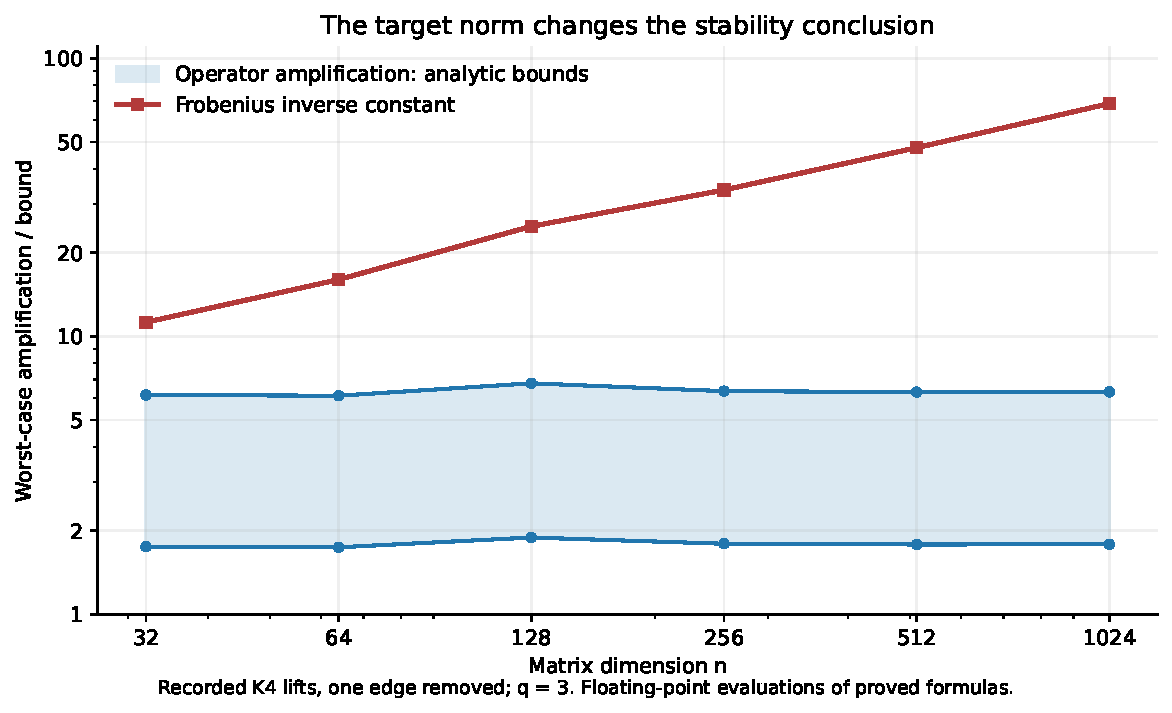
\includegraphics[width=0.88\linewidth]{norm_separation.pdf}
\caption{Three simplex actions on the recorded $K_4$ lifts after one edge is removed. The blue interval is the analytic lower/upper bound on operator amplification, evaluated numerically from the Green diagonal. The red curve is the Frobenius inverse constant from the smallest eigenvalue. These finite examples illustrate the proved all-size distinction; they do not prove it.}
\end{figure}

\paragraph{Failures retained.}
(1) The regular simplex design on an entire regular cover is noninjective: $I+A$ is an exact counterexample. (2) Rescaling a row leaves a congruent null matrix; the numerical residual was $5.9\cdot10^{-16}$. (3) The first full-support extension used a small perturbation and a small correction system; the star construction removes that restriction for the triangle family, but the general one-cycle version is retained because it has a broader local hypothesis. (4) A generic-rigidity argument establishes neither uniform constants nor finite-precision stability. (5) A scalar JSON serialization error interrupted the first star-diagnostic run; it was repaired by converting graph indices to Python integers, with no mathematical change. These are distinct from a falsification of the final theorems.

\section{Closest predecessors and the remaining obstruction}

Sparse Hessian compression and recovery from coloring-based seed matrices are established. Gebremedhin, Pothen, Tarafdar and Walther give star/acyclic-color recovery algorithms and analyze substitution error in Section 3.3, Theorem 3.1 \cite{hessian}. This note uses non-coordinate simplex probes and analyzes an absolute adversarial Frobenius input norm against an operator output norm. It does not claim the first stable sparse-Hessian recovery method.

Halikias and Townsend study structured recovery from matrix--vector products, including query complexity and a dimension lower bound (Lemma 2.2) \cite{halikias}. Amsel et al. prove optimal-order query bounds for relative Frobenius approximation to a prescribed sparsity pattern and explicitly discuss the operator-norm extension as an open direction in Section 6 \cite{amsel}. Their unknown matrix may have arbitrary off-pattern entries. Exact known support in the present theorem is a materially different assumption; this note does not solve that relative-approximation question. Gallmeier and Otto give randomized one-sided reconstruction for local row-subspace models, with a Frobenius approximation contract \cite{gallmeier}.

Graph resistance has prior roles in estimation. Chen, Xi and Yu relate entry-specific estimation of additive matrices to electrical flows and resistance in Theorem 4 \cite{chen}. The use of a Green function as an error invariant is therefore not itself a novelty claim. The scoped candidate contribution here is the exact simplex normal operator, its operator-norm criterion, and the full-support cycle-anchor construction. Whether any of these formulations already appears in the literature remains UNKNOWN.

\subsection{Why generic rigidity was insufficient}

For any finite $X\in\R^{n\times q}$ with nonzero rows, choose an invertible column transformation $R$ whose first column avoids all row-orthogonality hyperplanes. Then $XR=D[\one,p]$ with invertible diagonal $D$. Thus
\[
HX=0\quad\Longleftrightarrow\quad \Omega[\one,p]=0,
\qquad\Omega=DHD.
\]
The first equation fixes the stress diagonal; the others are equilibrium equations at the affine points $p_i\in\R^{q-1}$. This is an established rigidity/stress representation; Heaton's work is a recent nearby treatment of generic stresses \cite{heaton}. The argument itself is elementary. Its weakness for this task is quantitative: $D$ may be badly conditioned, and a nonzero generic minor may approach zero with graph size. The Green-diagonal calculation supplies exactly the norm-specific quantitative information that the generic representation omits.

\subsection{Precisely what remains open here}

\begin{enumerate}
\item \textbf{General support geometry.} Remove the closed-neighborhood simplex coloring and the isolated short-cycle interface while preserving three-query uniform operator stability on a substantially broader class of cubic supports. No such general theorem has been proved here. The exceptional complete graph $K_4$ cannot be recovered with three actions: for any $X\in\R^{4\times3}$, a nonzero $z\in\ker X^T$ gives the full-support null matrix $zz^T$.
\item \textbf{Approximate support.} If the true matrix is $H+R$, then $RX$ is additional data error. The elementary bound $\norm{RX}_{\F}\leq\norm R_{\op}\norm X_{\F}$ can grow as $\sqrt n$. The current theorem therefore supplies no dimension-free operator-relative approximation result.
\item \textbf{Numerical arithmetic.} The residual certificates above resolve one missing interface. An end-to-end implementation must still certify roundoff in the probe actions, local cycle measurements, residual evaluation, and solve, then compare total cost with coordinate coloring. Such a bound and comparison have not been supplied.
\item \textbf{Priority.} Obtain an independent theorem-by-theorem adversarial review and a more exhaustive comparison with non-coordinate Hessian seeds and stress-based reconstruction. No publication priority is asserted.
\end{enumerate}

The exact next investigation is to implement the residual-balanced solve with certified residual evaluation, measure the arithmetic and accuracy needed for a fixed operator-error target, and compare three-action reconstruction with the four-color isometric baseline. Use \eqref{eq:residual-l1} or \eqref{eq:balanced}, not an unbalanced residual tolerance. A second independent direction is the general-cubic-support question above. Neither a performance advantage nor that broader theorem is assumed in the current result.

\begin{thebibliography}{10}
\bibitem{corpus} Astra research knowledge, pinned revision \texttt{e606bfc587c76bdcae8b8fa3ec33e721efa2fbac}.
Entry file: \href{https://github.com/harjassand/astra-research-knowledge/blob/e606bfc587c76bdcae8b8fa3ec33e721efa2fbac/00_START_HERE.txt}{00\_START\_HERE.txt}.
Selected scientific contract: \href{https://github.com/harjassand/astra-research-knowledge/blob/e606bfc587c76bdcae8b8fa3ec33e721efa2fbac/research/2026-10-23-scientific-cycles/cycle-11/pro2/PROOF.md}{cycle-11/pro2/PROOF.md}. Read 23 October 2026.
\bibitem{bordenave} C. Bordenave, \emph{A new proof of Friedman's second eigenvalue Theorem and its extension to random lifts}, arXiv:1502.04482v4, 5 March 2019. Corollary 24, p. 31, checked directly. \url{https://arxiv.org/pdf/1502.04482v4}.
\bibitem{hessian} A. H. Gebremedhin, A. Pothen, A. Tarafdar and A. Walther, \emph{Efficient Computation of Sparse Hessians using Coloring and Automatic Differentiation}. Author manuscript, revision 21 March 2008; Section 3.3 and Theorem 3.1 read. DOI:10.1287/ijoc.1080.0286. \url{https://www.cs.purdue.edu/homes/apothen/Papers/hessian-coloring-joc.pdf}.
\bibitem{halikias} D. Halikias and A. Townsend, \emph{Structured matrix recovery from matrix-vector products}, arXiv:2212.09841v2, 29 May 2023. Introduction, Lemma 2.2 and noise discussion checked. \url{https://arxiv.org/pdf/2212.09841v2}.
\bibitem{amsel} N. Amsel, T. Chen, F. Duman Keles, D. Halikias, C. Musco and C. Musco, \emph{Fixed-sparsity matrix approximation from matrix-vector products}, arXiv:2402.09379v3, 26 March 2024. Problem 1 and Section 6 checked. \url{https://arxiv.org/pdf/2402.09379v3}.
\bibitem{gallmeier} E. Gallmeier and S. E. Otto, \emph{Efficient Approximation of Structured Linear Operators using Randomized One-Sided Queries}, arXiv:2610.07513v1, 5 October 2026. Introduction and Theorem 1 read. \url{https://arxiv.org/html/2610.07513v1}.
\bibitem{chen} Y. Chen, X. Xi and C. L. Yu, \emph{Entry-Specific Matrix Estimation under Arbitrary Sampling Patterns through the Lens of Network Flows}, arXiv:2409.03980v1, 6 September 2024. Abstract and Theorem 4 with proof read. \url{https://arxiv.org/html/2409.03980v1}.
\bibitem{heaton} A. Heaton, \emph{Generic Rigidity and the Grassmannian}, arXiv:2604.05442v3, 1 September 2026. Introduction and Lemma 3 checked; no theorem imported into the proofs above. \url{https://arxiv.org/html/2604.05442v3}.
\end{thebibliography}
\end{document}
